%\documentclass{article}
\documentclass[handout]{beamer}
%\usepackage{beamerarticle}
\usepackage{tikz}
\usetikzlibrary{arrows,shapes}

\author{S.Poss and A.Sailer}
\title{Luminosity spectrum measurement}
\subtitle{First results}

\mode<presentation>
{
   \setbeamertemplate{navigation symbols}{}
   \setbeamertemplate{footline}[frame number] 
}

\AtBeginSection[]
{
\begin{frame}<beamer>
\frametitle{Outline}
\tableofcontents[currentsection,currentsubsection]
\end{frame}
}


\begin{document}
\begin{frame}
\titlepage
\end{frame}
\begin{frame}
\frametitle{Outline}
\tableofcontents
% You might wish to add the option [pausesections]
\end{frame}
\tikzstyle{decision} = [diamond, draw, text badly centered, node distance=2.8cm]
\tikzstyle{block} = [rectangle, draw, text centered, rounded corners, text width=1.9cm, node distance=2.2cm]
\tikzstyle{autoblock} = [rectangle, draw, text centered, rounded corners, node distance=2.2cm]
\tikzstyle{line} = [draw, -triangle 90]
\tikzstyle{dline} = [draw, dashed, -triangle 90]
%\tikzstyle{cloud} = [draw, ellipse,fill=red!20, node distance=3cm,minimum height=2em]
\section{Introduction}
\begin{frame}
\frametitle{Luminosity spectrum}
Why it's important to know it:
\begin{itemize}
\item cross section measurements: Higgs, etc.
\item mass measurements: slepton analysis, etc.
\end{itemize}
What we want to ``measure'': set of parameters that describes the luminosity
spectrum.
\begin{itemize}
\item need a correct model, based on assumptions and existing Monte Carlo
samples
\item need a framework/procedure for parameter estimation
\item need data 
\end{itemize}
\end{frame}
\section{Obtaining data}
\begin{frame}
\frametitle{Obtaining data}
\begin{figure}[h]
\begin{tikzpicture}[scale=0.8,auto]
\matrix [column sep=7mm, row sep=4mm,ampersand replacement=\&]
{
%row1
\uncover<1->{\node [block] (money) {Get money};} \&
\uncover<2->{\node [block] (build) {Build machines};} \&
\uncover<3->{\node [block] (recdata) {Take Bhabha data};} \&
~\\
%row2
~ \&
~ \&
~ \&
\uncover<4->{\node [autoblock, color=red] (rec) {Reconstruction};} \\
%row3
~ \&
\uncover<5->{\node [block, text width=2.cm,] (gen) {Generation using GP and
BHWide};} \& \uncover<6->{\node [autoblock] (sim) {Simulate};} \&
~\\
};
\uncover<2->{\path [line] (money) -- (build);}
\uncover<3->{\path [line] (build) -- (recdata);}
\uncover<4->{\path [line] (recdata) -| (rec);}
\uncover<6->{\path [line] (gen) -- (sim);}
\uncover<7->{\path [line] (sim) -| (rec);}
\end{tikzpicture}
\end{figure}
\end{frame}

\section{Chosen model}
\begin{frame}
\frametitle{Chosen model}
Guinea pig data:
\centering
\includegraphics[width=9cm]{Reference}
\end{frame}
\begin{frame}
\frametitle{Chosen model}
Guinea pig data:
\centering
\includegraphics[width=9cm]{Reference_zoomed}
\end{frame}
\begin{frame}
\frametitle{Chosen model}
Depending on whether the beams emitted beamstrahlung: 
\begin{itemize}
  \item none (Peak): uniform distribution
  \item one only (Arm1): 1 BetaFunction $x^a(1-x)^b$
  \item other only (Arm2): 1 other BetaFunction
  \item both (Body): 2 other BetaFunctions
\end{itemize}
Every region is independent and has corresponding probability to happen.\\
~\\
Beam spread also leads to different effects:
\begin{itemize}
  \item peak (2 Beta Functions assumed to be independent)
  \item in each arms (2 other independent Beta functions), valid for the body
  too
\end{itemize}

\end{frame}
\begin{frame}
\frametitle{Why different beam spreads in the arms}
\begin{center}
\includegraphics[width=7cm]{E_vs_v_colz_electrons}\\
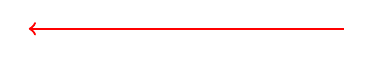
\begin{tikzpicture}[auto]
\draw [->, thick, color=red](2,0) -- (-2,0);
\end{tikzpicture}
\end{center}
A particle from the back (with lower energy) is more likely to
interact with a particle from the other beam that has emitted beamstrahlung.
\end{frame}

\begin{frame}
\frametitle{Chosen model: Beam spread}
\begin{tikzpicture}[auto]
\node[draw, node distance=2.2cm]{\includegraphics[width=10cm]{DeltaE_electron_fit_BetaFunction}};
\end{tikzpicture}
\end{frame}

\begin{frame}
\frametitle{Chosen model: Beam spread}
\begin{tikzpicture}[auto]
\node[draw, node distance=2.2cm]{\includegraphics[width=10cm]{DeltaE_electron_fit_BetaFunction_regions}};
\node[block, text width=2.9cm]{Tails obtained by convoluting with gaussian with
fixed width.};
\end{tikzpicture}
\end{frame}
\begin{frame}
\frametitle{Chosen model: Beam spread generated}
\includegraphics[width=10cm]{MCBeamSpread}
\end{frame}
\begin{frame}
\frametitle{Chosen model: Beamstrahlung}
Use the same working hypothesis as Andr\'e's thesis:\\
 Beta Function $x^a(1-x)^b$, where $a>0$ and $b<0$.\\
\begin{center}
\includegraphics[width=7cm]{BetaFunction_beamstrahlung}
\end{center}
\end{frame}

\begin{frame}
\frametitle{Chosen model: final model}
One event's probability:
\begin{equation}
P(E_1) = P(\Delta E,\textrm{BeamSpread})\times 
P(E,\textrm{Beamstrahlung})
\end{equation}
$E_1$ is a random variable of $P(E_1)$, and the individual componants depend
on the regions, picked randomly for every event.
\end{frame}

\begin{frame}
\frametitle{Chosen model: generated samples E1 vs E2}
\centering
\includegraphics[width=9cm]{StartingParameters}
\end{frame}
\begin{frame}
\frametitle{Chosen model: generated samples E1 vs E2}
\centering
\includegraphics[width=9cm]{StartingParameters_zoomed}
\end{frame}
\begin{frame}
\frametitle{Chosen model: Guinea Pig}
\centering
\includegraphics[width=9cm]{Reference_zoomed}
\end{frame}

\section{Fitting methods}
\begin{frame}
\frametitle{Fitting methods}
2 methods are available:
\begin{itemize}
\item Simple fit: dumb and easy, obvious method, but not CPU wise,
\item Reweighting fit: smart and elegant, not so obvious, but clearly affordable CPU wise.
\end{itemize}
~\\
Definition: \alert{$[p]_N$ is a set of parameter values} at the $N^{th}$
iteration, not a set of parameterisations: all iterations use the SAME
parametrisation.
\end{frame}
\section{Fitting}
\subsection{First method: Simple fit}
\begin{frame}
\frametitle{First method: Simple fit}
\begin{figure}[h]
  \begin{tikzpicture}[scale=2.8,auto]
\uncover<1-2>{\node [autoblock] (start) {\scriptsize Start: $[p]_0$};}
\uncover<2->{\node [block, below of=start, color=blue] (gen) {\scriptsize Generate Event with $[p]_N$: E1,E2};}
\uncover<3-10,12->{\node [autoblock, right of=gen] (bhwide) {\scriptsize BHWide};}
\uncover<4-10,13->{\node [autoblock, right of=bhwide] (sim) {\scriptsize Simulation};}
\uncover<5-10,14->{\node [autoblock, right of=sim] (rec) {\scriptsize Reconstruction};}
\uncover<6-10,15->{\node [block, below of=rec, color=red] (compare) {\scriptsize Compare with data: $\chi^2$};}
\uncover<7-10,16->{\node [decision, left of=compare, color=violet] (match)
{\scriptsize Minimum?};} \uncover<8-10,17->{\node [autoblock, below of=match] (done) {\scriptsize Done!};}
\uncover<9-11,18->{\node [block, below of=gen, color=magenta] (minim) {\scriptsize Minimizer: $[p]_N \rightarrow [p]_{N+1}$};}
\uncover<1-2>{\path [line] (start) -- (gen);}
\uncover<3-10,12->{\path [line] (gen) -- (bhwide);}
\uncover<4-10,13->{\path [line] (bhwide) -- (sim);}
\uncover<5-10,14->{\path [line] (sim) -- (rec);}
\uncover<6-10,15->{\path [line] (rec) -- (compare);}
\uncover<7-10,16->{\path [line] (compare) -- (match);}
\uncover<8-10,17->{\path [line] (match) -- node [near start] {\scriptsize yes} (done);}
\uncover<9-10,18->{\path [line] (match) -- node [near start] {\scriptsize no} (minim);}
\uncover<10-11,19->{\path [line] (minim) -- (gen);}
%\node (start) at (0,2) [draw] {Start};
%\node (gen) at (0,1) [draw] {Generate Event with $[P]_N$: E1,E2};
\end{tikzpicture}
\end{figure}
\end{frame}
\begin{frame}
\frametitle{First method: Simple fit}
Pros:
\begin{itemize}
\item logical
\item straight-foward to set up
\end{itemize}
Cons:
\begin{itemize}
\item Takes forever
\item all MC samples need to be reconstructed (1 reco per iteration)
\end{itemize}
~\\
\alert{Need better idea.}
\end{frame}

\subsection{Second method: Reweighting fit}
\begin{frame}
\frametitle{Understanding the reweighting fit}
\begin{itemize}
  \item A \alert{distribution} of an observable $=$ \alert{``probability''} for
  an event to happen with a given observable value. Observable can be e.g.
  $\{EB1,EB2\}$ for a given event%, in fact 1 event
  %$=\{E1,E2,\theta_1,\theta_2,E_{ECAL1},E_{ECAL2}\}$)
  \item If said distribution is built from a set of parameters' values
  $[p]$, then probabilities can be computed from that set
  \item Changing $[p]\to [p]'\Rightarrow$ change of the probabilities. This
  change is accounted by the ratio $\frac{P(\{EB1,EB2\},
  [p]')}{P(\{EB1,EB2\},[p])}$. This weight is applied individually to every
  event.
  \item Bhabha events are not only represented by $\{EB1,EB2\}$ but by
  $\{EB1,EB2,\theta_1,\theta_2,E_{ECAL1},E_{ECAL2},etc.\}$ where the
  $\{\theta_1,\theta_2,E_{ECAL1},E_{ECAL2},etc.\}$ set are reconstructed
  (measured) observables
\end{itemize}
\end{frame}
\begin{frame}
\frametitle{Second method: reweighting fit}
%Shown in fig.~\ref{fig:second}
%begin{figure}[h]
\begin{tikzpicture}[scale=.8,auto, remember picture]
\matrix [column sep=5mm,row sep=4mm,ampersand replacement=\&]{
%row1
\uncover<1>{\node [autoblock] (start) {\scriptsize Start};} \& 
~ \& 
~ \&
~ \\
%row2
\uncover<2->{\node [block, color=blue] (gen) {\scriptsize Generate Event with $[p]_0$: $E1$, $E2$, $P(E1,E2;[p]_0)$};} \&
\uncover<3-5>{\node [autoblock, node distance=2.7cm] (bhwide) {\scriptsize BHWide};} \&
\uncover<4-5>{\node [autoblock, node distance=2.5cm] (sim) {\scriptsize Simulation};} \&
\uncover<5->{\node [autoblock, node distance=2.7cm] (rec) {\scriptsize Reconstruction};} \\
%row3
\uncover<6->{\node [block, color=magenta] (minim) {\scriptsize Minimizer: $[p]_N \rightarrow [p]_{N+1}$};} \&
\uncover<7-13,15->{\node [block, text width=2.2cm, node distance=2.7cm] (compute) {\scriptsize Compute $P(E1,E2;[p]_{N+1})$ for all events};} \&
\uncover<8-13,16->{\node [autoblock, node distance=2.8cm] (weight) {\scriptsize $w = \frac{P(E1,E2;[p]_{N+1})}{P(E1,E2;[p]_{0})}$};} \&
\uncover<9-13,17->{\node [block, node distance=2.7cm] (weightrec) {\scriptsize Weight every event with its weight $w$};} \\
%row4
~ \& 
~ \& 
\uncover<11-13,19->{\node [decision, color=violet] (match) {\scriptsize
Minimum?};} \& \uncover<10-13,18->{\node [block, color=red] (compare) {\scriptsize Compare with data: $\chi^2$};}\\
%row5
~ \& 
~ \& 
\uncover<12-13,20->{\node [autoblock] (done) {\scriptsize Done!};} \& 
~ \\
};
\begin{scope}
\uncover<1>{\path [line] (start) -- (gen);}
\uncover<3-5>{\path [line] (gen) -- (bhwide);}
\uncover<4-5>{\path [line] (bhwide) -- (sim);}
\uncover<5>{\path [line] (sim) -- (rec);}
\uncover<6>{\path [line] (gen) -- (minim);}
\uncover<7-13,15->{\path [line] (minim) -- (compute);}
\uncover<8-13,16->{\path [line] (compute) -- (weight);}
\uncover<9-13,17->{\path [line] (weight) -- (weightrec);}
\uncover<10-13,18->{\path [line] (weightrec) -- (compare);}
\uncover<11-13,19->{\path [line] (compare) -- (match);}
\uncover<12-13,20->{\path [line] (match) -- node [near start] {\scriptsize yes} (done);}
\uncover<13,21->{\path [line] (match) -| node [very near start] {\scriptsize no} (minim);}
\uncover<9-13,17->{\path [dline] (rec) -- node [midway] {\scriptsize use} (weightrec); }
\end{scope}
\end{tikzpicture}
%\end{figure}
\end{frame}
\subsection{Status}
\begin{frame}
\frametitle{Current status}
Procedure for MC generation exists.\\
~\\
Data and MC samples share 
\begin{itemize}
  \item generator (BHWide)
  \item simulation (Mokka)
  \item reconstruction (Marlin)
\end{itemize}
$\to$ Forget about simu/reco effects for the moment, they will only smear
the distributions (systematics).\\
~\\
Fine tunning of fitting needed as there are many parameters (20): number of
bins, parameter ranges, etc.
\end{frame}


\section{Fit results}
\begin{frame}
\frametitle{Fit results so far}
\centering
\includegraphics[width=9cm]{final_res}\\
Tail well modelized, peak not perfect yet.
\end{frame}

\section{Next step: Bhabha events}
\begin{frame}
\frametitle{Bhabha events}
After discussions with JJ:
\begin{itemize}
  \item Bhabha events at large angles ($\theta > 7\deg$): cross section is
  10~pb.
  \item Corresponds to $\approx 30,000$ events reconstructible per day
\end{itemize}
$\Rightarrow$ statistics should not be an issue.\\
~\\
Will start simulation and reconstruction of MC and data samples.
\end{frame}
\section{Systematic effects}
\begin{frame}
\frametitle{Expected systematic effects}
From Model:
\begin{itemize}
  \item Beam spread: gaussian smearing is fixed
  \item Beam spread: validity range of BetaFunctions is fixed
\end{itemize}
  $\Rightarrow$ Study effect of fluctuation\\
\pause
From Simulation/reconstruction:
\begin{itemize}
  \item for the moment, same generator is used for data and MC: real life is
  another story
  \item same thing for the simulation: if the detector is different between
  simu and reality (and it's a fact), so are the MC/data. 
\end{itemize}
\pause
Physics effects:
\begin{itemize}
  \item effect of background contamination 
  \item detector resolution 
\end{itemize}
\end{frame}
\section{Conclusion}
\begin{frame}
\frametitle{Conclusion}
\begin{itemize}
  \item Framework is set up
  \item MC samples are created, need to be BHWided for generator level study,
  then Mokkaed, and then Marlined
  \item Idem for data sample
  \item Fit on existing samples show good progress
  \item Systematics will need more thoughts
\end{itemize}

\end{frame}
\appendix
\begin{frame}
\begin{center}
{\color{blue} Appendix}
\end{center}
\end{frame}
\section{Guinea pig correlations}
\begin{frame}
\frametitle{Are beam energies correlated?}
\includegraphics[width=9cm]{GPnominal_vs_GPmixed}
\end{frame}

\end{document}
